\documentclass{efd-lecture}

\begin{document}

\begin{frame}
  \titlepage{}
\end{frame}
\begin{frame}
  \frametitle{Outline}
  \tableofcontents{}
\end{frame}

\section{Introduction}

\begin{frame}
  \begin{itemize}
    \item Documentation is any communicable material that is used to \textit{\color{YellowOrange}describe}, \textit{\color{YellowOrange}explain} or \textit{\color{YellowOrange}instruct}
      regarding some attributes of an object, system or procedure,
      such as its \textit{\color{LimeGreen}parts}, \textit{\color{LimeGreen}assembly}, \textit{\color{LimeGreen}installation},
      \textit{\color{LimeGreen}maintenance} and \textit{\color{LimeGreen}use}.
    \item Documentation can be provided on paper, online, or on digital or analog media, such as audio tape or CDs. Examples are user guides, white papers, online help, and quick-reference guides.
    \item Paper or hard-copy documentation has become less common.
    \item Documentation is often distributed via websites, software products, and other online applications.
  \end{itemize}
\end{frame}

\section{JSON Schema}

\begin{frame}
  \frametitle{JSON Schema}
  \begin{itemize}
    \item JSON schema is JSON also
    \item The JSON document being validated or described we call the
      \textit{\color{YellowOrange} instance}, and the document containing the
      description is called the \textit{\color{GreenYellow} schema}.
  \end{itemize}
\end{frame}

\begin{frame}[fragile]
  \frametitle{Hello World}
  \begin{itemize}
    \item This accepts anything, as long as it’s valid JSON
      \mint[bgcolor=Black]{json}|{}|
    \item The most common thing to do in a JSON Schema is to restrict to a specific type. The \textit{\color{YellowOrange} type} keyword is used for that.
    \begin{minted}[bgcolor=Black]{json}
{ "type": "string" }
    \end{minted}
  \end{itemize}
\end{frame}

\begin{frame}[fragile]
  \frametitle{Declaring a JSON Schema}
  \begin{itemize}
    \item It's generally good practice to include it, though it is not required.
    \item The \textit{\color{YellowOrange} \$schema} keyword is used to declare
        that something is JSON Schema.
    \item Since JSON Schema is itself JSON, it's not always easy to tell when
        something is JSON Schema or just an arbitrary chunk of JSON.
  \end{itemize}
  \begin{minted}[bgcolor=Black]{json}
{ "$schema": "http://json-schema.org/draft-07/schema#" }
{ "$schema": "http://json-schema.org/draft/2019-09/schema#" }
  \end{minted}
\end{frame}

\begin{frame}[fragile]
  \frametitle{Declaring a unique identifier}
  \begin{itemize}
    \item It is also best practice to include an
      \textit{\color{YellowOrange} \$id} property as a unique identifier for
      each schema.
    \item For now, just set it to a URL at a domain you control, for example:
  \end{itemize}
  \begin{minted}[bgcolor=Black]{json}
{ "$id": "http://yourdomain.com/schemas/myschema.json" }
  \end{minted}
\end{frame}

\begin{frame}
  \frametitle{Annotations}
  \begin{itemize}
    \item JSON Schema includes a few keywords,
      \textit{\color{YellowOrange}title},
      \textit{\color{YellowOrange}description},
      \textit{\color{YellowOrange}default},
      \textit{\color{YellowOrange}examples} that
      \textbf{\color{LimeGreen} aren’t strictly used for validation},
      but are used to describe parts of a schema.
    \item The \textit{\color{Yellow}title} and
      \textit{\color{Yellow}description} keywords must be strings.
    \item A ``title'' will preferably be short, whereas a ``description'' will provide
      a more lengthy explanation about the purpose of the data described by
      the schema.
    \item The \textit{\color{Cyan}default} keyword specifies a default
      value for an item.
  \end{itemize}
\end{frame}

\begin{frame}[fragile]
  \frametitle{String}
  \begin{minted}[bgcolor=Black]{json}
{ "type": "string" }
  \end{minted}
  \begin{itemize}
    \item Length
    \begin{itemize}
      \item
        The length of a string can be constrained using the
        \textit{\color{LimeGreen}minLength} and
        \textit{\color{YellowOrange}maxLength} keywords.
      \item For both keywords, the value must be a non-negative number.
    \end{itemize}
    \item Regular Expressions
    \begin{itemize}
      \item The \textit{\color{YellowOrange}pattern} keyword is used to restrict
        a string to a particular regular expression.
    \end{itemize}
  \end{itemize}
\end{frame}

\begin{frame}
  \frametitle{String (cont'd)}
  \begin{itemize}
    \item Format
    \begin{itemize}
      \item The \textit{\color{Cyan}format} keyword allows for basic
        semantic validation on certain kinds of string values that are
        commonly used.
      \begin{itemize}
        \item Dates and times
        \item Email addresses
        \item Hostnames
        \item IP Addresses
        \item \ldots
      \end{itemize}
    \end{itemize}
  \end{itemize}
\end{frame}

\begin{frame}[fragile]
  \frametitle{Numeric types}
  \begin{itemize}
    \item The integer type is used for integral numbers.
    \begin{minted}[bgcolor=Black]{json}
{ "type": "integer" }
    \end{minted}
    \item
      The number type is used for any numeric type, either integers or
      floating point numbers.

    \begin{minted}[bgcolor=Black]{json}
{ "type": "number" }
    \end{minted}
  \end{itemize}
\end{frame}

\begin{frame}
  \frametitle{Numeric types (Cont'd)}
  \begin{itemize}
    \item Multiples
    \begin{itemize}
      \item
        Numbers can be restricted to a multiple of a given number, using the
        \textit{\color{YellowOrange}multipleOf}.

      \item It may be set to any positive number.
    \end{itemize}
    \item Range
    \begin{itemize}
      \item
        Ranges of numbers are specified using a combination of the
        \textit{\color{YellowOrange}minimum} and
        \textit{\color{YellowOrange}maximum} keywords

    \end{itemize}
  \end{itemize}
\end{frame}

\begin{frame}[fragile]
  \frametitle{Object}
  \begin{itemize}
    \item Objects are the mapping type in JSON.
    \begin{minted}[bgcolor=Black]{json}
{ "type": "object" }
    \end{minted}
    \item Properties
    \begin{itemize}
      \item
        The properties (key-value pairs) on an object are defined using the
        \textit{\color{YellowOrange}properties} keyword.
      \item
        The value of \textit{\color{YellowOrange}properties} is an object,
        where each key is the name of a property and each value is a JSON
        schema used to validate that property.
    \end{itemize}
  \end{itemize}
\end{frame}

\begin{frame}[fragile]
  \frametitle{Object (Cont'd)}
  \scriptsize
  \begin{minted}[bgcolor=Black]{json}
{
  "type": "object",
  "properties": {
    "number":      { "type": "number" },
    "street_name": { "type": "string" },
    "street_type": { "type": "string",
                     "enum": ["Street", "Avenue", "Boulevard"]
                   }
  }
}
  \end{minted}
\end{frame}

\begin{frame}
  \frametitle{Object (Cont'd)}
  \begin{itemize}
    \item
      The \textit{\color{Purple}additionalProperties} keyword is used
      to control the handling of extra stuff

    \item
      properties whose names are not listed in the
      \textit{\color{YellowOrange}properties} keyword.

    \item
      By default any additional properties are
      \textit{\color{LimeGreen}allowed}

    \item
      If \textit{\color{Purple}additionalProperties} is an object,
      that object is a schema that will be used to validate any additional
      properties not listed in properties.

  \end{itemize}
\end{frame}

\begin{frame}[fragile]
  \scriptsize
  \begin{minted}[bgcolor=Black]{json}
{
  "type": "object",
  "properties": {
    "number": { "type": "number" },
    "street_name": { "type": "string" },
    "street_type": { "enum": ["Street", "Avenue", "Boulevard"] }
  },
  "additionalProperties": { "type": "string" }
}
    </code></pre>
    <pre><code class="lang-json">
{
  "type": "object",
  "properties": {
    "number": { "type": "number" },
    "street_name": { "type": "string" },
    "street_type": { "enum": ["Street", "Avenue", "Boulevard"] }
  },
  "additionalProperties": false
}
  \end{minted}
\end{frame}

\begin{frame}
  \frametitle{Object (Cont'd)}
  \begin{itemize}
    \item
      By default, the properties defined by the properties keyword are
      \textit{\color{RubineRed}not required}.
    \item
      The \textit{\color{YellowOrange}required} keyword takes an array of
      zero or more strings.
  \end{itemize}
\end{frame}

\begin{frame}[fragile]
  \frametitle{Object (Cont'd)}
  \begin{minted}[bgcolor=Black]{json}
{
  "type": "object",
  "properties": {
    "name":      { "type": "string" },
    "email":     { "type": "string" },
    "address":   { "type": "string" },
    "telephone": { "type": "string" }
  },
  "required": ["name", "email"]
}
  \end{minted}
\end{frame}

\begin{frame}[fragile]
  \frametitle{Array}
  \begin{itemize}
    \item Arrays are used for ordered elements.
    \item In JSON, each element in an array may be of a different type.
    \begin{minted}[bgcolor=Black]{json}
{ "type": "array" }
    \end{minted}
    \item
      List validation is useful for arrays of arbitrary length where each item
      matches the \textit{\color{Yellow} same schema}.
    \item
      For this kind of array, set the
      \textit{\color{YellowOrange} items} keyword to a single schema that
      will be used to validate all of the items in the array.
  \end{itemize}
\end{frame}

\begin{frame}[fragile]
  \frametitle{Array (cont'd)}
  \begin{minted}[bgcolor=Black]{json}
{
  "type": "array",
  "items": {
    "type": "number"
  }
}
  \end{minted}
\end{frame}

\begin{frame}[fragile]
  \frametitle{Example}
  \scriptsize
  \begin{minted}[bgcolor=Black]{json}
{
  "$schema": "http://json-schema.org/draft-07/schema#",
  "title": "Product",
  "type": "object",
  "properties": {
    "id": {
      "type": "number",
      "description": "Product identifier"
    },
    "name": { "type": "string" },
    "price": { "type": "number", "minimum": 0 },
    "tags": {
      "type": "array",
      "items": { "type": "string" }
    },
    "stock": {
      "type": "object",
      "properties": {
        "warehouse": { "type": "number" },
        "retail": { "type": "number" }
        }
      }
   }
}
  \end{minted}
\end{frame}

\begin{frame}[fragile]
  \frametitle{Example (Cont'd)}
  \begin{minted}[bgcolor=Black]{json}
{
  "id": 1,
  "name": "Foo",
  "price": 123,
   "tags": [
    "Bar",
    "Eek"
  ],
  "stock": {
   "warehouse": 300,
   "retail": 20
  }
}
  \end{minted}
\end{frame}

\begin{frame}[fragile]
  \frametitle{Example}
  \scriptsize
  \begin{minted}[bgcolor=Black]{json}
{
  "$schema": "http://json-schema.org/draft-07/schema#",
  "$id": "https://gitlab.snapp.ir/shared-services/jamaal/dpn/contract.json",
  "type": "object",
  "required": [
    "from",
    "to",
    "accept_rate",
  ],
  "properties": {
    "from": {
      "type": "string",
      "format": "date-time"
    },
    "city_id": {
      "type": "integer"
    },
    "to": {
      "type": "string",
      "format": "date-time"
    },
    "accept_rate": {
      "type": "number",
      "minimum": 0,
      "maximum": 100
    }
  }
}
  \end{minted}
\end{frame}

\section{Swagger}

\begin{frame}
  \begin{itemize}
    \begin{block}{}
      The OpenAPI Specification (OAS) defines a \textit{\color{YelloOrange}standard},
      \textit{\color{LimeGreen}language-agnostic} interface
      to RESTful APIs which allows both humans and computers to discover and understand
      the capabilities of the service \textbf{\color{RubineRed}without} access to source code, documentation,
      or through network traffic inspection.
    \end{block}
    \begin{block}{}
      When properly defined, a consumer can understand and interact with the remote service
      with a minimal amount of implementation logic.
    \end{block}
  \end{itemize}
\end{frame}

\section{AsyncAPI}

\begin{frame}
  \frametitle{Event-Driven Architectures}
  \begin{itemize}
    \item In most cases, Event-Driven Architectures (EDAs) are broker-centric.
    \item A message broker (or ``broker'') is a piece of infrastructure in charge of receiving messages and delivering them to those who have shown interest.
    \item A publisher (a.k.a.\ producer) is an application that sends messages to the broker.
    \item A subscriber (a.k.a.\ consumer) is an application that connects to the broker, manifests an interest in a certain type of messages,
      and \textit{\color{YellowOrange}leaves} the connection open so the broker can push messages to them.
  \end{itemize}
  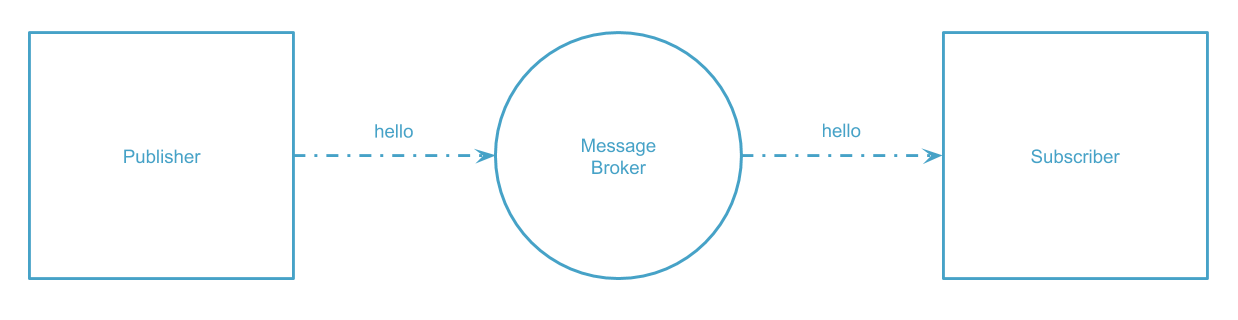
\includegraphics[width=\textwidth]{./img/simple-event-driven.png}
\end{frame}

\begin{frame}[fragile]
  \frametitle{Hello World}
  \begin{minted}[bgcolor=Black]{yaml}
asyncapi: 2.2.0
info:
  title: Hello world application
  version: '0.1.0'
channels:
  hello:
    publish:
      message:
        payload:
          type: string
          pattern: '^hello .+$'
  \end{minted}
\end{frame}

\begin{frame}[fragile]
  \frametitle{Hello World (Cont'd)}
  \begin{block}{}
    The first line of the specification starts with the document type \textit{\color{YellowOrange} asyncapi} and the version (2.2.0).
    This line doesn't have to be the first one,
    but it's a recommended practice.
  \end{block}
\end{frame}

\begin{frame}[fragile]
  \frametitle{Hello World (Cont'd)}
  \begin{block}{}
    The \textit{\color{YellowOrange} info} object contains the minimum required information about the application.
    It contains the \textit{\color{YellowGreen} title}, which is a memorable name for the API, and the version. While it's not mandatory,
    it's strongly recommended to change the \textit{\color{YellowGreen} version} whenever you make changes to the API\@.
  \end{block}
\end{frame}

\begin{frame}[fragile]
  \frametitle{Hello World (Cont'd)}
  \begin{block}{}
    The channels section of the specification houses all of the mediums where messages flow through. For example,
    some systems use topic, event name or routing key.
    Different kinds of information flow through each channel similar to the analogy of TV channels.
  \end{block}
\end{frame}

\begin{frame}
  \begin{block}{}
    This is the payload of the message that the Hello world application is subscribed to.
    You can publish the message to the hello channel and the Hello world application will receive it.
  \end{block}
\end{frame}

\begin{frame}
  \frametitle{Channels}
  \begin{description}
    \item[subscribe] A definition of the \textsc{\color{YellowOrange}Subscribe} operation, which defines the messages produced by the application and sent to the channel.
    \item[publish] A definition of the \textsc{\color{LimeGreen}Publish} operation, which defines the messages consumed by the application from the channel.
    \item[bindings] A map where the keys describe the name of the \textit{\text{Cyan}protocol} and the values describe protocol-specific definitions for the channel.
    \item[parameters] A map of the parameters included in the \textbf{\color{Purple} channel name}.
  \end{description}
\end{frame}

\begin{frame}[fragile]
  \frametitle{Channels (Cont'd)}
  \scriptsize
  \begin{minted}[bgcolor=Black]{yaml}
description: This channel is used to exchange messages about users signing up
subscribe:
  summary: A user signed up
  message:
    description: A longer description of the message
    payload:
      type: object
      properties:
        user:
          $ref: "#/components/schemas/user"
        signup:
          $ref: "#/components/schemas/signup"
bindings:
  amqp:
    is: routingKey
    exchange:
      name: myExchange
      type: topic
      durable: true
      autoDelete: false
      vhost: /
  \end{minted}
\end{frame}

\begin{frame}[fragile]
  \frametitle{Channels (Cont'd)}
  \scriptsize
  \begin{minted}[bgcolor=Black]{yaml}
user/{userId}/signup:
  parameters:
    userId:
      description: Id of the user
      schema:
        type: string
  subscribe:
    message:
      $ref: "#/components/messages/userSignedUp"
  \end{minted}
\end{frame}

\begin{frame}[fragile]
  \frametitle{Operation}
  \begin{itemize}
    \item Describes a publish or a subscribe operation. This provides a place to document how and why messages are sent and received.
  \end{itemize}
  \begin{description}
    \item[tags] A list of tags for API documentation control. Tags can be used for \textit{\color{YellowOrange} logical grouping} of operations.
    \item[description] A verbose explanation of the operation.
    \item[bindings] A map where the keys describe the name of the protocol and the values describe protocol-specific definitions for the operation.
    \item[message] A definition of the message that will be published or received by this operation. Map containing a single oneOf key is allowed here to specify multiple messages.
      However, a message MUST be valid only against one of the message objects.
  \end{description}
\end{frame}

\begin{frame}[fragile]
  \frametitle{Operation (Cont'd)}
  \begin{minted}[bgcolor=Black]{yaml}
operationId: registerUser
summary: Action to sign a user up
description: A longer description
tags:
  - name: user
  - name: signup
  - name: register
message:
  headers:
    type: object
    properties:
      applicationInstanceId:
        description: Unique identifier for a given instance of the publishing application
        type: string
  payload:
    type: object
    properties:
      user:
        $ref: "#/components/schemas/userCreate"
      signup:
        $ref: "#/components/schemas/signup"
bindings:
  amqp:
    ack: false
  \end{minted}
\end{frame}

\section{Go}

\begin{frame}
  \frametitle{How to Run?}
  \begin{itemize}
    \item List the service dependencies
    \item Have a docker-compose with these dependencies
  \end{itemize}
\end{frame}

\begin{frame}
  \frametitle{Comment}
  \begin{itemize}
    \item Have comments on exported \textit{\color{YellowOrange}Fields}, \textit{\color{LimeGreen}Methods},
      \textit{\color{Cyan}Functions} and \textit{\color{RubineRed}Structs}.
    \item Rule 1: Comments should not duplicate the code.
    \item Rule 2: Good comments do not excuse unclear code.
    \item Rule 3: If you can’t write a clear comment, there may be a problem with the code.
  \end{itemize}
\end{frame}

\begin{frame}
  \frametitle{Comment (Cont'd)}
  \begin{itemize}
    \item Rule 4: Comments should dispel confusion, not cause it.
    \item Rule 5: Explain unidiomatic code in comments.
    \item Rule 6: Provide links to the original source of copied code.
    \item Rule 7: Include links to external references where they will be most helpful.
    \item Rule 8: Add comments when fixing bugs.
    \item Rule 9: Use comments to mark incomplete implementations.
  \end{itemize}
\end{frame}

\begin{frame}[fragile]
  \frametitle{Comment (Cont'd)}
  \begin{minted}[bgcolor=Black]{kotlin}
if (x > 3) {
   …
} // if
  \end{minted}
\end{frame}

\begin{frame}[fragile]
  \frametitle{Comment (Cont'd)}
  \begin{minted}[bgcolor=Black]{kotlin}
private static Node getBestChildNode(Node node) {
    Node n; // best child node candidate
    for (Node node: node.getChildren()) {
        // update n if the current state is better
        if (n == null || utility(node) > utility(n)) {
            n = node;
        }
    }
    return n;
}
  \end{minted}
\end{frame}

\begin{frame}[fragile]
  \frametitle{Comment (Cont'd)}
  \begin{minted}[bgcolor=Black]{kotlin}
final Object value = (new JSONTokener(jsonString)).nextValue();
// Note that JSONTokener.nextValue() may return
// a value equals() to null.
if (value == null || value.equals(null)) {
    return null;
}
  \end{minted}
  \begin{minted}[bgcolor=Black]{kotlin}
/** Converts a Drawable to Bitmap.
  via https://stackoverflow.com/a/46018816/2219998. */
  \end{minted}
\end{frame}

\begin{frame}[fragile]
  \frametitle{Comment (Cont'd)}
  \scriptsize
  \begin{minted}[bgcolor=Black]{kotlin}
// http://tools.ietf.org/html/rfc4180 suggests that CSV lines
// should be terminated by CRLF, hence the \r\n.
csvStringBuilder.append("\r\n");
  \end{minted}
  \begin{minted}[bgcolor=Black]{kotlin}
// NOTE: At least in Firefox 2, if the user drags outside of the browser window,
// mouse-move (and even mouse-down) events will not be received until
// the user drags back inside the window. A workaround for this issue
// exists in the implementation for onMouseLeave().
@Override
public void onMouseMove(Widget sender, int x, int y) { .. }
  \end{minted}
\end{frame}

\begin{frame}
  \frametitle{Have everything on Git}
  \begin{itemize}
    \item \textbf{\color{RubineRed}Don't} relay on Environment variables because they don't have any documentation or history.
    \item \textbf{\color{RubineRed}Don't} store keys with Persons, they will forget it.
  \end{itemize}
\end{frame}

\section{Confluence}

\begin{frame}
  \frametitle{Do's and Don'ts}
  \begin{itemize}
    \item Use it for high-level architectures and meeting notes.
    \item \textbf{\color{RubineRed}Don't} store code-related things because they will be out of sync soon.
  \end{itemize}
\end{frame}

\section{Conclusion}

\begin{frame}
  \begin{center}
  
\includegraphics[height=\textheight]{./img/cartoon-1.png}
  \end{center}
\end{frame}

\begin{frame}
  \begin{center}
  
\includegraphics[height=\textheight]{./img/cartoon-2.png}
  \end{center}
\end{frame}

\begin{frame}
  \frametitle{References}
  \begin{itemize}
    \item https://stackoverflow.blog/2021/12/23/best-practices-for-writing-code-comments/
    \item https://www.asyncapi.com/ (Mohammad Nasr)
    \item https://swagger.io/
    \item http://json-schema.org/
  \end{itemize}
\end{frame}

\end{document}
